\documentclass[11pt]{article}
\usepackage[margin=1in]{geometry}
\usepackage[T1]{fontenc}
\usepackage{lmodern,microtype,amsmath,amssymb,booktabs,graphicx,hyperref,xcolor}
\hypersetup{colorlinks=true,linkcolor=blue!55!black,urlcolor=blue!55!black}
\title{\texttt{infl\_ens}: Influencer-Game Routing for Specialized SLMs}
\author{Project summary}
\date{\today}
\begin{document}
\maketitle
\begin{abstract}
\texttt{infl\_ens} asks whether small language-model adapters can specialize through
a mathematically structured competition for data. It transfers the influencer's game---
a spatial game in which agents compete for a resource distribution---to alignment:
resources are prompts, agents are LoRA adapters, and their positions lie in a learned
safety trait space. A router allocates prompts, SFT changes the adapters, and positions
are re-estimated. This is a controlled research hypothesis about specialization, not yet
a finished alignment solution. Current runs show clear \emph{routing} specialization,
but mixed end-to-end model-quality results; that gap is the central question.
\end{abstract}

\section{The project in one minute}
Clone a base SLM several times and place the clones in a low-dimensional map of prompts.
Prompts are resources. A clone near a prompt receives more of that training data, but
competes with nearby clones. After training the clones on allocated data, refresh their
positions and repeat:
\[
\text{corpus}\rightarrow\text{trait positions}\rightarrow\text{routing}\rightarrow
\text{LoRA SFT}\rightarrow\text{updated positions}.
\]
The desired outcome is a routed ensemble of complementary specialists rather than
nearly identical fine-tunes trained on one pooled mixture.

For mechanistic interpretability, the trait coordinates are not claimed to be literal
features inside a transformer. They are an \emph{external causal state abstraction}:
a benchmark-supervised summary used to intervene on each adapter's training
distribution. The project tests whether that intervention produces detectable
specialization in routing, cross-perplexity, and held-out benchmark NLL.

\section{The source theory}
The supplied paper, \emph{Learning Dynamics of the Influencer's Game in Resource
Landscapes}, studies $N$ agents choosing positions $x_i$. Resources have traits $b$ and
distribution $B(b)$. Agent $i$ has influence $f_i(x_i,b)$ and receives a proportional
share:
\begin{equation}
G_i(\mathbf{x},b)=\frac{f_i(x_i,b)}{\sum_{j=1}^{N}f_j(x_j,b)},\qquad
u_i(\mathbf{x})=\sum_b B(b)G_i(\mathbf{x},b).
\label{eq:game}
\end{equation}
The game is constant-sum. This repository uses a Gaussian influence kernel,
\begin{equation}
f_i(x_i,b)=\exp\!\left[-\tfrac12(x_i-b)^\mathsf{T}\Sigma^{-1}(x_i-b)\right],
\end{equation}
with $\Sigma=\sigma^2I$ when isotropic. Large $\sigma$ means broad competitive reach
(generalism); small $\sigma$ means a narrow niche (specialism).

Under suitable log-concavity conditions, the paper establishes a unique symmetric Nash
equilibrium. With Gaussian influence, it is the resource-weighted mean. In one dimension
the first stability boundary is
\begin{equation}
\sigma_0^*=\sqrt{\frac{N-2}{N-1}}\,\sigma_B,
\label{eq:threshold}
\end{equation}
where $\sigma_B$ is resource spread. Above this threshold, gradient dynamics return
agents to a shared generalist position. Below it, the symmetric state can lose stability
and form specialist clusters, cycles, and smaller competitive subgames. The paper also
reports the same qualitative bifurcation picture under independent Q-learning.

The alignment transfer is simple: a multi-modal prompt landscape should allocate
different regions to different adapters when the router is narrow enough. The caveat is
important: SFT does not literally execute the game's spatial gradient flow. The code's
theory-versus-SFT experiments exist to test this proposed bridge.

\section{What the repository implements}
\subsection{A learned safety trait space}
The \texttt{data} package turns labeled benchmark families into a common coordinate
system. Present axes cover harm (BeaverTails), hallucination (HaluEval), jailbreak
behavior (JBB-Behaviors or ToxicChat), privacy (AI4Privacy), over-refusal (OR-Bench),
prompt injection, and policy violation (Do-Not-Answer). Text is embedded with a
sentence-transformer or Hugging Face encoder; learned label-derived directions project
embeddings into $[0,1]^L$. Corpus density becomes the empirical resource distribution.

\begin{figure}[p]
\centering
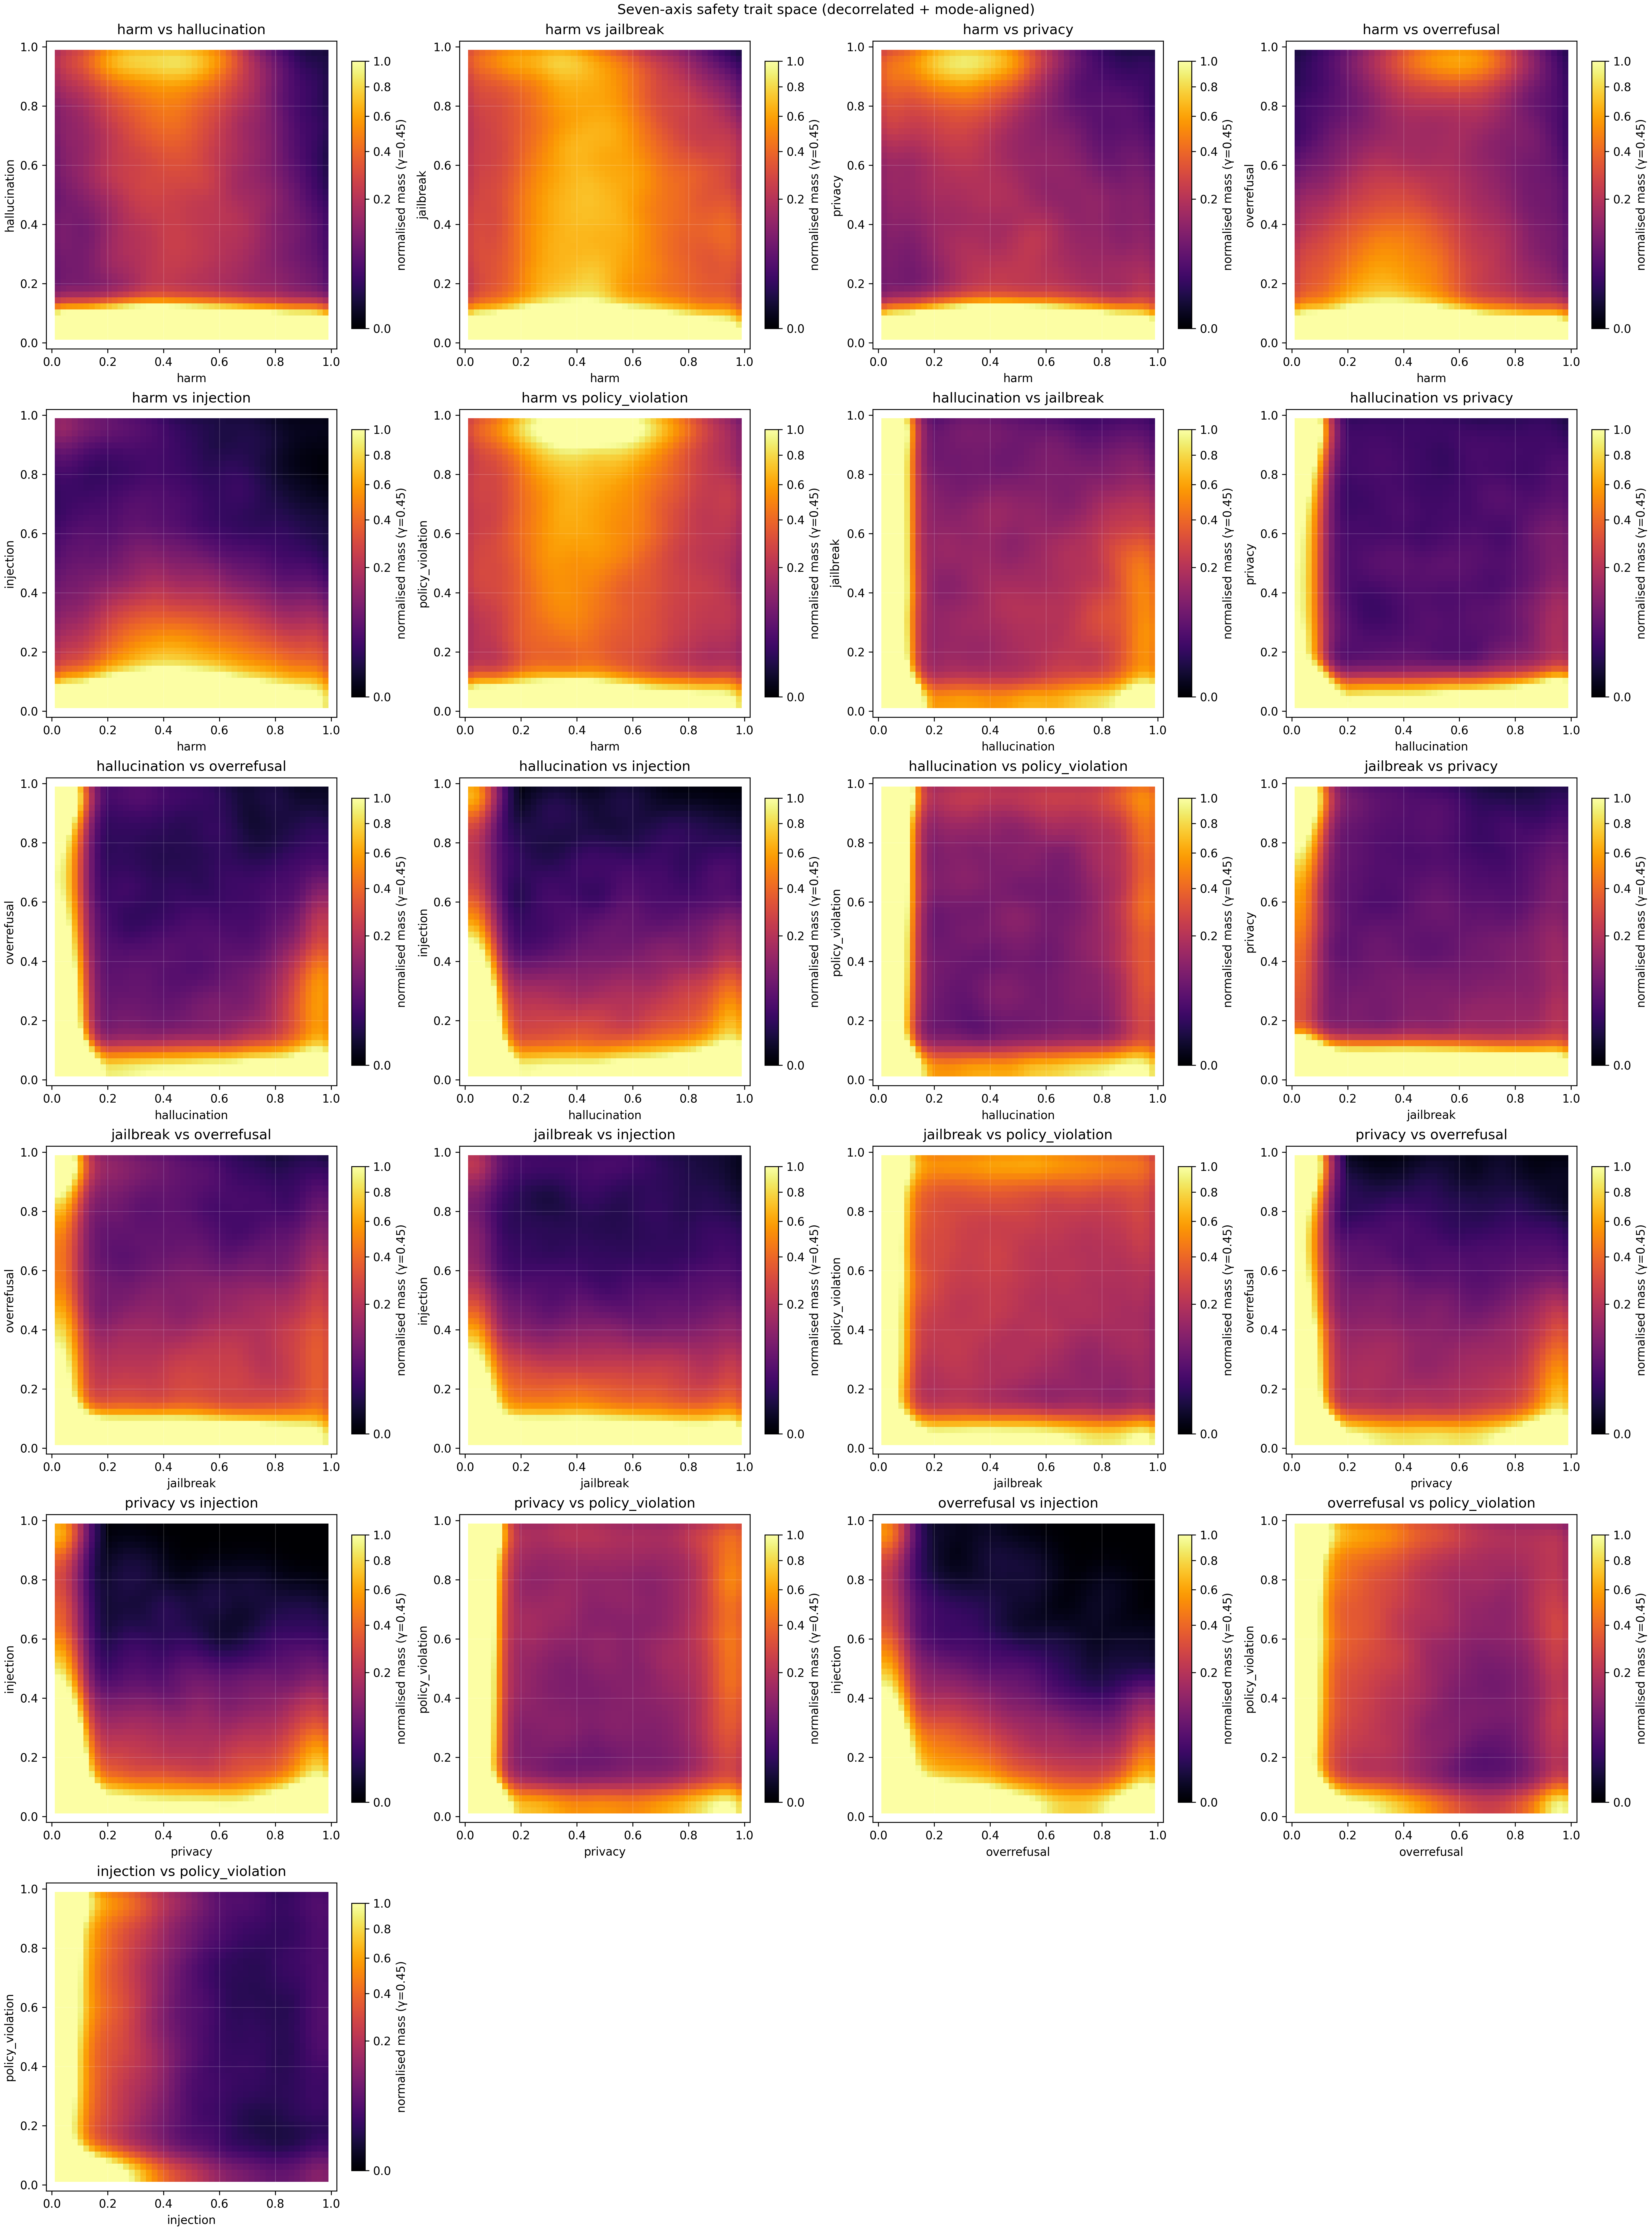
\includegraphics[height=.72\textheight,keepaspectratio]{../../scripts/figures/seven_axis_safety_resource_separated.png}
\caption{Pairwise slices of a seven-axis safety resource landscape generated by this
repository. Bright regions are prompt-dense locations in an external learned trait map,
not claimed model-internal features. This multi-modal geometry makes routing inspectable
and supplies the resource landscape for the game.}
\label{fig:resource}
\end{figure}

\subsection{Game-theoretic routing and LoRA training}
The \texttt{inflgame.router} package implements Equation~\ref{eq:game}: stable Gaussian
influence, allocation $G$, expected utility, and analytic utility gradients. Theory-only
runs optimize positions by gradient ascent. Closed-loop runs dispatch real prompts to
actual adapters.

\emph{Proportional routing} assigns a prompt in proportion to $G_i$.
\emph{Strategic routing} uses $G_i(1-G_i)$, the factor in the strategic gradient: it
de-emphasizes examples an agent already dominates and emphasizes contested examples.
The training package then runs SFT for each router agent, saves LoRA adapters under
\texttt{results/<run>/agents/}, and refreshes positions from held-out projected prompts.
It supports both cumulative and fresh-per-round LoRA, pooled-replay baselines, and
pair-merge experiments that reduce two trained clones to one served expert.

Three objects must remain distinct: \textbf{trait position} (the router's geometric
summary), \textbf{adapter parameters} (the actual transformer changes), and
\textbf{evaluation behavior} (NLL and specialist probes). Theory directly describes the
first; the scientific question is whether it causally organizes the second enough to
improve the third.

\section{How to read the current evidence}
The repo contains synthetic/theory-only routers, two- and three-axis safety spaces,
four- and six-agent LoRA loops, fixed-theory AI4Privacy studies, and seven-axis
pair-merge experiments. Evaluation reports mean next-token negative log likelihood
(NLL) on chat-formatted benchmark splits. Lower NLL means higher probability for a
reference continuation; it is useful for specialization diagnostics but not a complete
safety or helpfulness metric.

The strongest positive result is geometric and attributional. In one recorded seven-axis
run, the winning route matched benchmark type: the privacy expert won 858/1,000
AI4Privacy examples, the hallucination expert 825 HaluEval examples, the harm expert
623 BeaverTails examples, the policy expert 699 Do-Not-Answer examples, and the
over-refusal expert 586 OR-Bench examples. This supports meaningful data specialization
rather than arbitrary partitioning.

The end-to-end result is deliberately more cautious. In that run's flat routing
diagnostic, the pooled baseline had NLL 1.947, learned expected routing had 1.989, and
an oracle choice among experts had 1.916. The ensemble contains potentially useful
complementary experts, but the geometric router has not yet consistently converted that
complementarity into a win over pooled training. Candidate causes include an insufficient
trait map, a mismatch between NLL-optimal and influence-optimal routing, pair-merge
dilution, or SFT dynamics that differ from the assumed position dynamics.

\section{Why it is interesting for mechanistic interpretability}
\begin{itemize}
\item \textbf{Controlled curriculum interventions:} changing $\sigma$, initialization,
or routing policy changes the data distribution while holding base model and SFT fixed.
\item \textbf{Predicted phase changes:} Equation~\ref{eq:threshold} motivates a
collapse-to-specialize transition rather than merely asserting that diversity helps.
\item \textbf{Several observable levels:} geometry (positions/allocation), behavior
(NLL/benchmark scores), and parameters or representations (LoRA deltas/activations).
\item \textbf{Useful counterfactuals:} pooled replay, fixed-theory positions, random
versus theory initialization, proportional versus strategic routing, and corner ablations.
\end{itemize}
An informative next study would match examples per adapter while changing only their
trait-space curriculum. It could compare LoRA-delta similarity, layerwise activation
differences on each benchmark, and whether a linear probe for an external trait
coordinate becomes more separable in the expected specialist. A compelling result would
connect a known curriculum intervention, a behavioral niche, and a localized parameter
or representational change.

\section{Caveats and next steps}
\begin{enumerate}
\item \textbf{The theorem is not about transformers.} It proves properties of a spatial
game; SFT is a proposed realization that needs empirical fidelity checks.
\item \textbf{External axes are imperfect proxies.} Labels and embeddings can confound
topic, style, difficulty, and response format, so axis-separability diagnostics matter.
\item \textbf{NLL is limited.} It is not refusal quality, robustness, calibration, or
adversarial safety; behavioral metrics are needed before strong alignment claims.
\item \textbf{Routing is the bottleneck.} The oracle-versus-router gap motivates a
learned or calibrated router while retaining the game as a prior or regularizer.
\item \textbf{Attribution is decisive.} Use existing 2-by-2 controls, matched compute,
multiple seeds, and held-out splits to identify what actually causes a gain.
\end{enumerate}



\section{Bottom line}
\texttt{infl\_ens} turns a theory of competitive niche formation into an experimental
design for SLM specialization. Its router already finds semantically sensible niches, but
those niches do not automatically outperform a well-trained pooled model. Explaining or
closing that gap---with attributional controls and parameter/representation-level
measurements---is the central next experiment.

\paragraph{Source.} Based on the supplied Lovett and Fu draft, \emph{Learning Dynamics
of the Influencer's Game in Resource Landscapes}, and the repository state inspected on
\today. \href{https://www.dropbox.com/scl/fi/ui1pp36tm9mo1rh61wiki/public_facing_draft.pdf?rlkey=ybb9j0ekqlvwsy3puibwojnuf&dl=0}{Supplied paper PDF}.
\end{document}
